\chapter{Languages}
\label{languages}
The preceding section described a representation for programs which is suitable for any language. To define a particular language in this framework involves defining three aspects of the language.

The \emp{abstract syntax} of the language defines what nodes may appear in a program, and in what relationship to each other. In \Meta, abstract syntax is defined by a program in the \keyword{grammar} language. The grammar program is first and foremost a specification which defines what programs are (syntactically) valid. 

Every language must have a \emp{semantics} that gives its programs meaning. While there are any number of ways to specify semantics, or indeed to make use of languages and programs with only ill-defined semantics, the approach pursued here is that of one or more kernel languages and syntax extension. The example of Lisp shows this to be a successful strategy, so the experimental question is how well it applies in this new setting. When a grammar defines a node type, it may also define the semantics of the construct by means of a reduction to a more primitive construct.

With abstract syntax and semantics taken care of, both the Lisper and the Programming Language Theorist have all they need and will go happily on their ways. However, we would like to go further than that, so one more element is needed. \emp{Concrete syntax} is what the user reads and writes. The goal is to take advantage of the new approach to do things with concrete syntax that are impractical or impossible to do with textual source code. In \Meta, the concrete syntax of each type of node is given as a reduction to a \emp{presentation language}.

%
% Grammars
%
\section{Grammars}
\label{grammars}
Thus the grammar defines all three aspects of the language. The abstract syntax is defined \emp{prescriptively}, by determining what programs are legal. Both the semantics and concrete syntax are defined \emp{operationally}, as declarations of what reduced program and what visual representation will be derived from each source node.

\subsection{Abstract Syntax}
A program is \emp{valid} with respect to a \emp{grammar} if all of its node's types, values, and references comply with certain restrictions imposed by the grammar. For each node type, a grammar specifies:
\begin{enumerate}
\item Zero or more \emp{abstract types}, which are types for which the type being introduced is a \emp{sub-type}.
\item Whether the node's value should be an boolean, integer, string, sequence, or map.
\item For an integer-valued node, a range of legal values.
\item For a sequence node, the number and (abstract) type of expected child nodes.
\item For a map node, the expected attributes and the (abstract) types of nodes that may inhabit each of them.
\item When a child/attribute is a reference, the type of the expected (abstract) type of the referenced node.
\end{enumerate}

Abstract types lend some modularity to the grammar. A new subtype of any abstract type can be introduced later without changing any existing definition, and nodes with the new type can appear as children of nodes of the previously-defined types. Note: these simple types are entirely nominal---there is no inheritance of any kind, the type is meant exclusively to record the intended meaning of each node, and to guide the grammar in applying the rules of the abstract syntax.

Note that all these properties except the last are local in the sense described earlier---checking them requires inspecting only a single node and its immediate children. Checking the type of the node pointed to by a reference requires being able to inquire about the type of a node which may be anywhere in the program. However, this information is easily extracted up front to a map of types for all nodes in the tree, so this one non-local check seems to be worth including in the standard checker.

A grammar so-defined is not capable of specifying every interesting property of a language. That is, not every syntactically valid program is correct. Depending on the nature of the language being defined, additional, more ambitious specifications can define additional properties (e.g. proper use of lexically-scoped variables or type safety). The abstract syntax is meant to be an easily-defined first step, and indeed in some sense it \emp{is} the language (e.g. a Java program with type errors is just that, but a program that fails to adhere to the basic syntactic structure of Java doesn't seem to rate being called a Java program at all.)


\subsection{Reductions}
A grammar may supply one or two reductions for each node type. These reductions are code fragments which are used to construct reduction functions (see section \ref{reduction}) which take a program in the source language defined by the grammar and reduce it to a derived program. Using a meta-programming approach, the reductions are economical and simple to define, but the full host language is available for use in reductions when needed.

\begin{figure}[ht]
	\begin{center}
	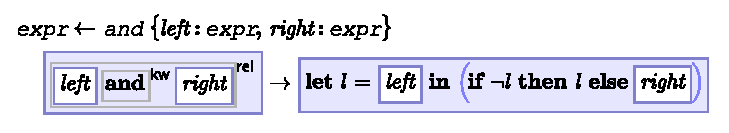
\includegraphics[scale=0.8]{src/image/and.pdf}
	\end{center}
	
	Taken from the grammar for the \Meta\ core language. \keyword{and} is a subtype of the abstract type \keyword{expr}, and has two required attributes, \emp{left} and \emp{right}, both \keyword{expr}s. On the left is the presentation reduction, which puts the string ``and'' in keyword style between the two expressions. An \keyword{and} node reduces to an expression which evaluates the left argument, tests to see if is a ``false'' value, returns it if not, and otherwise evaluates the right argument and returns that. This kind of short-circuiting evaluation returning the first false value is commonly used in scripting languages\cite{python-and}\cite{clojure-and}\cite{javascript}.
	
	\caption{Declaration of the \keyword{and} node of the core language.}
	\label{fig-and}
\end{figure}

A \keyword{display} reduction (shown on the left in Figure \ref{fig-and}) reduces a node to a presentation language node. This reduction will always be present except in certain special cases which will be described later.

An \keyword{expand} reduction is used to reduce a node in preparation for evaluation or execution, and therefore defines the semantics of the node. The result of this reduction is either a node in the \emp{target language}, or else a node that will itself be reduced, eventually to a target language node. The declaration of a node type does not provide an \keyword{expand} reduction if the node's semantics is defined externally; in that case the un-reduced node is already in target-language syntax.

It is easy to define a reduction that fails to terminate (by producing a node of equal size), or which ``blows up'' (by producing a larger, but no more reduced, node). However, this is mostly a problem in the early stages of language definition when core constructs are being defined on top of one another; once a usable core is available, most extensions build on that in a simple way. Anyway, once language definition is part of the development process, it should no longer be so surprising that problems can arise at that level. Because you are your own language vendor, you can simply fix it; it's not like finding a bug in your C++ compiler, which you may have no capability to fix.

Thus the abstract syntax, semantics, and concrete syntax of every language construct are defined together in a simple, declarative style. Therefore, each language construct is self-documenting. This flavor will be maintained in more interesting examples to come.

%
% Kernel languages:
%

\section{Kernel Languages}
A \emp{kernel language} is one whose nodes have some fixed, pre-defined semantics (typically, they can be evaluated, yielding some specified result with some specified side effects). A complete language is built by \emp{extending} a kernel language with additional nodes whose semantics is defined in terms of reduction to (ultimately) the kernel language.

Any language can act as a kernel language in \Meta. If the kernel language is of a more conventional type, say Java, all the constructs of that language have to be defined as primitives. Additional constructs could then be defined via reduction to ordinary Java syntax. After reduction, the target program would be processed by a Java compiler to produce an executable. Thus a language like Java is a suitable kernel language, but hardly a convenient one.

One kernel language, the \emp{host kernel language}, is designed to be much more simple to implement and use. It is the glue that makes the system work; for example the reductions themselves are written in it. Requirements for the host kernel language include:
\begin{enumerate}
\item Be in some sense minimal but sufficient, so that everything else can be done via extensions of it.
\item Be a meta-language, able to consume and produce nodes.
\item Fit well with the ``functional'' approach to nodes and trees.
\item Be easily implemented and easily integrated into a running application.
\end{enumerate}

In section \ref{host}, we'll describe the host kernel language of \Meta\ and how it fulfills these requirements.

The idea of a very minimal kernel language with a core language built on top of it is of course inspired by the Lisp family of languages. In particular, in Scheme\cite{scheme}, only a handful of \emp{special forms} are pre-defined, and all other language constructs are defined ``in the language'' in terms of macros which expand into the special forms. A similar approach is used for more didactic purposes in Mozart\cite{mozart}, at least in \emp{defining} the language, although it isn't clear that the implementation actually works this way.

%
% Presentation languages:
%

\section{Presentation Languages}
The nodes of a \emp{presentation} language cast program elements in visual terms. A presentation language should be independent of the particular syntax of any one language, but might be suited to a particular family of related languages. Crucially, the presentation language must be flexible enough to represent any conceivable construct that might be added to the source language. This is achieved by providing composable elements in the presentation language that can be combined in new ways to create new concrete syntax.

A presentation language is concrete in that it represents the program as it is presented to the user, however it is somewhat abstracted from the details of rendering characters and pixels. The reduction from source to presentation language is therefore quite direct and simple. Once the program is reduced to the presentation language, lower-level processing takes care of the details of rendering. This lower-level processing is common to all languages using the same presentation language, and does not need to be extended in the typical course of using (and extending) a source language.

To serve the needs of different kinds of languages, multiple presentation languages could be defined, such as a ``flowing text'' language for documents, a ``grid'' language for spreadsheet-like programs, a ``flowchart'' language for state machines, data flow programs, and regular expressions, and so forth. In \Meta, a single presentation language is currently implemented.

\subsection{The \keyword{expr} Language}

\Meta's \keyword{expr} language is well-suited to representing the expressions that make up the declarative portion of a typical modern programming language. It can also reproduce much of the familiar notation of algebraic expressions. An \keyword{expr} program is a tree made up of \emp{box} nodes. Each box node occupies a rectangular area of the rendering surface and always encloses the areas occupied by any child boxes. Several kinds of boxes are available in \keyword{expr}.

An \emp{atom} is a box that renders a sequence of characters and/or symbols using the normal spacing for text. Several types of atoms are available, each conveying what kind of entity the characters are meant to represent. When atoms are reduced to lower-level nodes, a distinctive typographical treatment is applied to each, as shown in Table \ref{tab-atoms}. The list of atom types is meant to be expanded to serve the needs of any conceivable source language; the effort to add a new type is typically small (most simply specify a font and/or face), and in any case the total number of types in any one language is probably limited to a dozen or so, with much in common across languages, so we conjecture that the universe of useful atom types is not much larger than what \keyword{expr} currently provides. 


\begin{table}

	\begin{center}
	\begin{tabular}{llll}
	Type & Treatment & Examples & Typical use
	\\
	\hline
	\keyword{keyword}
	 & boldface
	 & \keyword{true}
	 & fixed language syntax
	\\ & & \keyword{if} &   % Ugly hack! how to do proper multi-line cells in tabular env.?
	\\
	\hline
	\keyword{var}
	 & italic
	 & $x$
	 & names (user-provided or generated)
	\\ & & $g$ & 
	\\ & & $\mathit{fib}$ & 
	\\
	\hline
	\keyword{num}
	 & \textit{none}
	 & 1
	 & numerical literals
	\\ & & 2.0 & 
	\\ & & 3,000 & 
	\\
	\hline
	\keyword{string}
	 & sans serif
	 & \textsf{abc} 
	 & character literals (note special
	\\
	 & & \textsf{Hello,\textvisiblespace world} &  % open box: \u2423
	  treatment of the space character)
	\\
	%\hline
	%\keyword{name}
	% & boldface, italic
	% & \textbf{\emp{a}}
	% & name literals
	%\\ & & \textbf{\emp{foo}} & 
	%\\
	\hline
	\keyword{mono}
	 & monospaced
	 & \texttt{nil}
	 & external references
	\\ & & \texttt{cons} & 
	\\
	\hline
	\keyword{prod}
	 & monospaced, italic
	 & \texttt{\emp{expr}}
	 & node types in grammars
	\\ & & \texttt{\emp{left}} & 
	\\
	\hline
	\keyword{symbol}
	 & \textit{none}
	 & $\to$
	 & mathematical symbols
	\\ & & $\in$ & 
	\\ & & $\sum$ & 
	\\
	\hline
	\end{tabular}
	\end{center}
	
	\vspace{6pt}
	Note: the actual character content of each type of atom is arbitrary, except \keyword{symbol}, which handles a pre-defined set of available symbol.

	\caption{Types of atoms in the \keyword{expr} language.}
	\label{tab-atoms}
\end{table}

The diversity of atom types provides a measure of visual sophistication for programs, with a very small effort on the part of the language designer. Simply by identifying a visual style for each piece of syntax, some information about the meaning of each node is conveyed to the programmer. The particular treatment is meant to match the readability and high aesthetic standards of the pseudocode that might be found in a journal article or a good Computer Science textbook, and may be judged by the reader by inspecting any of the figures in this paper, most of which were captured directly from the prototype editor as vector graphics. The rendering of these fonts on screen at relatively low resolution of 100 dots per inch or less is not really optimal, but given the trend toward more dense displays (as of late 2010, laptop displays approaching 150 dpi are common and handheld devices can be much higher than that), it is likely that acceptable rendering of multiple fonts even at small sizes will soon be quite achievable. In any case, the actual choice of how to present each type of atom is unrestricted; a more conventional approach would be to use just a few fonts and instead use color to distinguish different elements in the conventional ``syntax-highlighting'' manner.\cite{lexx} These issues have been explored heavily in the field of Integrated Development Environments, but few published studies seem to exist. One reference is Harward, et al.\cite{insitu}

%A similar idea leads to the \emp{syntax-coloring} behavior of many text editors, with a more cartoonish and less elegant result (see Figure \ref{fig-syntax-coloring}). In \Meta, using a single color for all syntax allows color differences to be used for other purposes.

%\begin{figure}[t]
%  \begin{center}
%  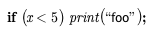
\includegraphics[scale=0.8]{src/image/if.png}  % 72dpi/0.8 = 88.75, actually
%  
%  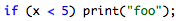
\includegraphics[scale=0.8]{src/image/if-text.png}
%  \end{center}
%  
%  A simple Java expression, rendered by \Meta\ and by a typical programmer's editor (TextMate), both at 90dpi. Note that the colored version is rendered using sub-pixel anti-aliasing, which looks better on screen than on the page.

%  \caption{Typographically-rich notation compared to ``syntax coloring.''}
%  \label{fig-syntax-coloring}
  
%\end{figure}

\emp{Composite} boxes contain child boxes which they arrange in a certain way. A \emp{sequence} is a horizontal arrangement of nodes separated by a certain amount of space. There are a handful of sequence types, each implying a certain amount of inter-node space. The amount of space is a visual indication of how tightly the sub-expression represented by the sequence binds, as we'll discuss in the next subsection. A \keyword{scripted} node contains a \emp{nucleus} and one or both of a \keyword{sub}- and \keyword{super}-script node. \emp{Special signs} are similar to composites but also draw a glyph surrounding the child node(s). Examples are \keyword{radical} and \keyword{fraction}, used in particular mathematical contexts.

A \keyword{group} node draws a pair of grouping symbols around a content node. Available symbols include parentheses, various kinds of brackets, $\lfloor\mathit{floor}\rfloor$, $\lceil\mathit{ceiling}\rceil$, and $|\mathit{magnitude}|$. All these symbols expand vertically to visually surround their contents; this variation is aesthetically pleasing, but also provides a visual cue which helps the reader to match up the paired symbols.

An \keyword{embed} node encloses its contents in a visual indication of being a separate unit, contained within the surrounding context. A \keyword{disembed} node has the opposite effect, showing its contents as being part of the outer level of code. These are used in the rendering of quotations, and have been seen already in the example reductions in Figure \ref{fig-and}.

Because the \keyword{expr} language preserves the hierarchical structure of expressions and specifies the visual layout of each sub-expression, it's possible for the system to identify cases where the nesting of expressions could lead to confusion, and to insert parentheses automatically in these cases. This is done \emp{after} the reduction of the program to the \keyword{expr} language, so it's applied consistently to any language construct, without special effort at the point of definition of a node. 

The \keyword{expr} language provides enough levels of spacing (four) to handle a moderately complex expression without parentheses. For example, in the expression
\begin{center}
%$$\keyword{if} \:\ \: x \: < \: y + 4! \:\ \: \keyword{then} \:\ \: \dots$$ 
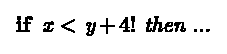
\includegraphics{src/image/space.pdf}
\end{center}  % too much space here (actually part of the pdf?), and an unfortunate page break, currently.
the factorial operator binds most tightly ($!$, no space), then addition is performed ($+$, indicated by a thin space), then comparison ($<$, medium space), and finally the conditional (\keyword{if}, thick space). Examples of how this works will be presented later.



\keyword{expr} provides no real support for sequences of statements, or for larger constructs such as methods, classes and modules. These larger constructs pose different layout problems, such as how to handle indentation and whether lines should be wrapped and how. Therefore, it would make sense to implement a second presentation language, say \keyword{program}, which would include nodes for these concepts. In \Meta, these constructs can be implemented somewhat awkwardly using the lower-level presentation language described in section \ref{view}.

%
% Extending...
%

\section{Extending a Language}
The grammar language, host language, and presentation language work together to support the definition of new language constructs. A grammar (i.e.\ a program in the \keyword{grammar} language) consists of a collection of node type declarations (\keyword{grammar} nodes), each containing reductions (which are host language nodes). A display reduction in turn contains quoted nodes in a presentation language (e.g.\ \keyword{expr}), while an ``expand'' reduction quotes nodes in the target language (which may be the host language or some other target language). This is only the start; a grammar can define syntax for embedding subtrees in yet more languages, such as when a regular expression sub-language is added as an extension to a general-purpose language. This extensive embedding is the key to economy of expression in \Meta.\footnote{And it inspired the name \Meta. A grammar is a meta-language, so the grammar for grammars is a meta-meta-language. Warning: this kind of thing is fun when it works, but it can be a mind-twisting chore to get it bootstrapped.}

\temp{When it's desirable to keep track of what source node gave rise to a given target node, the reduction can record the labels of each pair of source and target node, forming a kind of mapping between the parallel trees. For this to work, the reduction function needs to operate strictly on the single node it's given, and not reach into any child node. This in turn places some constraints on the way the source program is constructed: each node (along with any environment) must bear sufficient information to identify the correct reduction.}

Because a grammar is a \Meta\ program, the same tools for syntax extension are available for use in grammars, so the \keyword{grammar} language should be viewed as a starting point. It is meant to be general enough to define typical languages, to handle most common needs for defining syntax, and to serve as a kernel language for grammars.

As an example, consider the variety of 2-argument, infix operators that we may wish to define. If defined in terms of the kernel grammar language, each declaration will echo the definition of \keyword{and} shown in Figure \ref{fig-and}, varying only in the symbol used to represent the operator, and the name of a function to invoke. This kind of duplication is a clear opportunity for language extension, as shown in Figures \ref{fig-binary}.

\begin{figure}[th]
	\begin{center}
	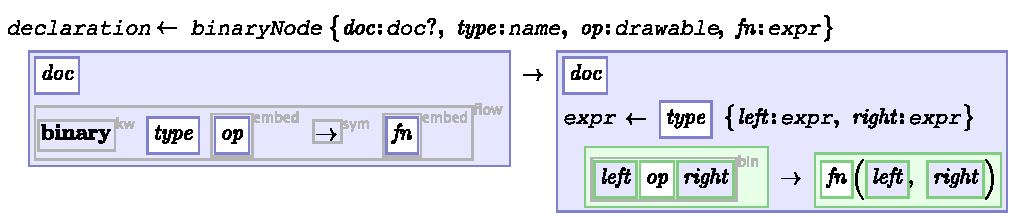
\includegraphics[scale=0.8]{src/image/binaryNode.pdf}
	\end{center}

	The display reduction (the blue, quoted box on the left) for these declarations mimics the regular node declaration syntax but with several fixed elements and just four embedded attributes. The expansion on the right is a quoted declaration, which will be evaluated to produce an ordinary node declaration.
  
	\caption{Definition of \keyword{binaryNode} as an extension of the grammar syntax.}
	\label{fig-binary}
\end{figure}

\begin{figure}[th]
	\begin{center}
	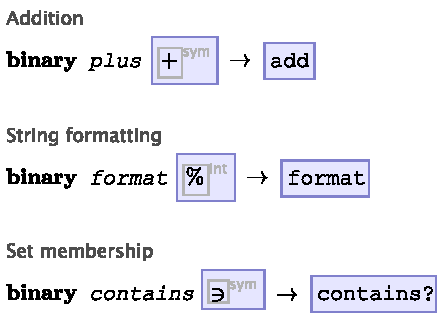
\includegraphics[scale=0.8]{src/image/binary.pdf}
	\end{center}

  \caption{Some infix operators defined using \keyword{binaryNode}.}
  \label{fig-binary-examples}
\end{figure}

Note that the presentation for the new node visually approximates the original declaration, but it is in fact much simplified. This simplification becomes apparent when you edit one of these nodes---only the four embedded elements are actually present in the AST (and therefore editable), and the rest of the visualization is just a fixed scaffolding provided by the reduction. The expanded declaration contains about 16 nodes. Like much syntax extension, the new node embodies the well-known goal of eliminating code duplication\cite{dry}. Still, the meaning is clear at a glance because the presentation is easily recognized by its visual resemblance to the lower-level form. As seen in Figure~\ref{fig-binary-examples}, node types defined using this new syntax are significantly simplified.
